\section{The Trisection of an Angle}

\begin{teo}
The trisection of the angle by an unmarked ruler and compass alone
is {\em in general} not possible.
\end{teo}


This problem, together with {\em Doubling the Cube}, {\em Constructing the
regular Heptagon} and {\em Squaring the Circle} were posed by the Greeks in
antiquity, and remained open until modern times.

The solution to all of them is rather inelegant from a geometric
perspective. No geometric proof has been offered [check?],
however, a very clever solution was found using fairly basic
results from extension fields and modern algebra.

It turns out that trisecting the angle is equivalent to solving
a cubic equation. Constructions with ruler and compass may
only compute the solution of a limited set of such equations,
even when restricted to integer coefficients. In particular,
the equation for $\theta = 60$ degrees cannot be solved by
ruler and compass and thus the trisection of the angle is not
possible.

It is possible to trisect an angle using a compass and a ruler marked
in 2 places.

Suppose $X$ is a point on the unit circle such that $\angle XOE$ is
the angle we would like to ``trisect''. Draw a line $AX$ through a
point $A$ on the $x$-axis such that $|AB| = 1$ (which is the same as
the radius of the circle), where $B$ is the intersection-point of the
line $AX$ with the circle.

\begin{figure}
\center
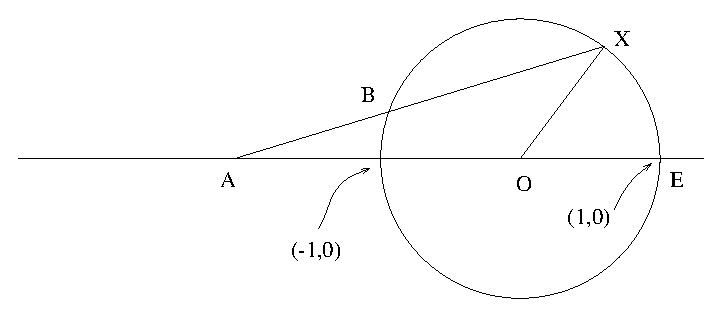
\includegraphics{figs/tri}
\caption{Trisection of the Angle with a marked ruler}
\end{figure}


Let $\theta$ be $\angle BAO$.
Then $\angle BOA = \theta$, and $\angle XBO = \angle BXO= 2\theta$

Since the sum of the internal angles of a triangle equals $\pi$
radians ($180$ degrees) we have $ \angle XBO + \angle BXO + \angle BOX
= \pi$, implying $4 \theta + \angle BOX = \pi$.  Also, we have that
$\angle AOB + \angle BOX + \angle XOE = \pi$, implying $\theta +\angle
BOX + \angle XOE = \pi$. Since both quantities are equal to $\pi$
we obtain

\[ 4 \theta + \angle BOX = \theta +\angle BOX + \angle XOE \]

From which

\[ 3 \theta = \angle XOE \]

follows. QED.


